\documentclass{article}
\usepackage{iclr2025_conference,times}

\input{math_commands.tex}

\usepackage[hidelinks]{hyperref}
\usepackage{url}
\usepackage{graphicx}
\usepackage{amsmath}
\usepackage{booktabs}
\usepackage{listings}
\usepackage{xcolor}

\lstdefinestyle{pylike}{
    basicstyle=\small\ttfamily,
    keywordstyle=\color{blue!70!black}\bfseries,
    commentstyle=\color{gray!70!black}\itshape,
    stringstyle=\color{teal!60!black},
    showstringspaces=false,
    breaklines=true,
    frame=single,
    framesep=4pt,
    rulecolor=\color{black!30},
    columns=fullflexible,
}
\lstset{style=pylike}

\title{SoniSphere-LoRA: Instruction-Driven Environmental Speech Synthesis on
CosyVoice3 via Flow-Stage FiLM Conditioning}

\author{ZHE CHEN \quad LINGYU YANG}

\newcommand{\fix}{\marginpar{FIX}}
\newcommand{\new}{\marginpar{NEW}}

\begin{document}

\maketitle

\begin{abstract}
We investigate how to extend a pretrained text-to-speech (TTS) backbone with
instruction-driven reverberation control: given a natural-language prompt such as
``speaking in a large hall'', the system should synthesize speech with
the corresponding reverberation characteristics, while preserving the
backbone's existing voice-cloning and style-instruction abilities. Building on
\textbf{Fun-CosyVoice3-0.5B-2512} (LLM~+~flow~+~vocoder), we report a four-phase
exploration. Phase~1 attempts direct supervised fine-tuning of the LLM stage with
three learning-rate variants and consistently fails: small learning rates leave
the model unmoved, while larger ones cause catastrophic memorization of the
training set. Phase~2 isolates the bottleneck via a bypass-LLM diagnostic,
showing that the speech-token codec actually preserves $\sim 70\%$ of the reverberant
energy, so the failure is in the LLM \emph{generation} of reverb-bearing tokens
rather than in the codec or the downstream Flow / HifiGAN. Phase~3 trains an
independent reverb classifier ($92\%$ dev accuracy) for objective evaluation.
Phase~4 introduces \textbf{Flow-FiLM}: a $\sim$40k-parameter conditioning layer
on the Flow stage that maps tokenized instructions to per-feature
$(\gamma,\beta)$ modulation. Activating this layer requires three coupled
engineering changes---\emph{clean-token alignment}, \emph{conds=0
leakage removal}, and \emph{per-parameter $100\times$ learning rate}---which we
ablate. The resulting system reaches $4/4$ on a coarse room-size benchmark and
$6/7=86\%$ on composite-instruction test cases, while voice cloning and
style following remain unaffected. We share the data pipeline, model patches,
and evaluation harness.
\end{abstract}

\section{Introduction}

Modern neural TTS systems such as VALL-E, Voicebox, and CosyVoice generate
high-quality, near-studio-clean speech and devote significant engineering to
\emph{removing} ambient noise and reverberation. Many practical applications,
however, require speech that sounds as if it was \emph{recorded in a specific
acoustic scene}: game NPC voicing, audiobook scene immersion, AR/VR spatial
audio, and post-production for short-form video all benefit from being able to
say ``put this voice in a cathedral'' rather than ``clean up this voice.''

We study whether a strong, frozen TTS backbone can be \emph{extended} with such
controllability through an instruction interface. Concretely, given text $T$
and a natural-language environment instruction $I$ (e.g., ``speaking in a
large hall with long reverb''), we want to generate a waveform $S = f(T,I)$
that preserves linguistic content, speaker timbre, and the backbone's existing
style-instruction behaviour, while honouring the acoustic semantics of $I$.

The contribution of this report is twofold. First, we present a systematic
exploration that locates the bottleneck of the obvious approach---LLM-stage
supervised fine-tuning---using three failure modes (collapse, under-fitting,
U-shape rebound) and a token-level diagnostic. Second, we describe a minimal
intervention that succeeds: a feature-wise linear modulation
(FiLM~\citep{perez2018film}) layer of $\sim$40k parameters injected at the
Flow stage, paired with three data-pipeline changes that together unlock its
training signal. The final system retains all original capabilities of
CosyVoice3 while passing a 4-class room-size benchmark and a 7-case
composite-instruction test at $86\%$.

\paragraph{Related work.}
Our work builds on neural TTS backbones that condition acoustic generation on
both text and an external embedding. WaveNet-style
vocoders~\citep{shen2018natural,ping2019clarinet}, FastSpeech-family acoustic
models~\citep{ren2019fastspeech,ren2021fastspeech2}, and recent codec /
flow-matching backbones such as CosyVoice2 and Voicebox~\citep{le2023voicebox}
have made high-quality multi-speaker zero-shot TTS practical. Most recently,
codec language models such as VALL-E and its successors~\citep{wang2023neuralcodecLM,
chen2024valle2,han2024valler,song2024ellav,du2024vallt,wang2024maskgct}, and
instruction-following systems such as
MaskGCT and Spark-TTS~\citep{wang2025sparktts}, have extended the conditioning
interface to natural-language style instructions (emotion, dialect, speaking
speed). In contrast, the dimension we target---explicit \emph{environmental}
control through instructions---has received limited attention in
instruction-driven TTS, partly because the backbones already aim at studio
quality. The closest analogues are room-aware speech enhancement and RIR-based
data augmentation, but these treat reverb as a nuisance rather than as a
controllable output. We also borrow conditioning ideas from FiLM
\citep{perez2018film} and from data-augmentation pipelines that use OpenSLR~28
RIRs~\citep{ko2017rir}.

\section{Background and Problem Setup}

\subsection{The CosyVoice3 backbone}

CosyVoice3 organizes synthesis into three sequential stages. Given the user
inputs (text $T$, instruction $I$, reference voice $W_p$), the inference path
is:
\begin{equation}
T,I,W_p \;\xrightarrow{\text{LLM (Qwen2 0.5B)}}\; \mathbf{c} \in \{1,\dots,V\}^{L}
\;\xrightarrow{\text{Flow (DiT)}}\; \mathbf{m} \in \mathbb{R}^{F\times L'}
\;\xrightarrow{\text{HifiGAN}}\; s \in \mathbb{R}^{T_s},
\end{equation}
where $\mathbf{c}$ is a sequence of \emph{discrete speech tokens} from the
\texttt{speech\_tokenizer\_v3} codec ($V = 4096$, frame rate
$\sim 50$\,Hz), $\mathbf{m}$ is an $80$-dim mel spectrogram, and $s$ is the
final 24\,kHz waveform. Speaker timbre is injected via a CAM++-style
embedding extracted from $W_p$; style instructions are processed by the LLM as
additional text tokens prepended to the generation context.

The natural place to inject ``room reverberation'' is therefore one of three
stages: (i) the LLM, by training it to emit reverb-bearing tokens conditioned on
$I$; (ii) the Flow, by adding a conditioning input that modulates the
token-to-mel mapping; or (iii) the HifiGAN, by allowing $I$ to alter the
mel-to-wave step. We pursue (i) first (Phase~1), conclude that the
information-density of the token channel makes it ill-suited to the task
(Phase~2--3), and finally settle on (ii) (Phase~4) as the right intervention
point.

\subsection{Problem statement}

We define the \emph{instruction-driven environmental TTS} task as follows. Let
$\mathcal{R}=\{r_1,\dots,r_K\}$ be a finite set of acoustic-scene categories
(e.g., $\{$clean, small\_room, medium\_room, large\_room$\}$), each described
by a small bag of paraphrastic natural-language instructions. Given training
triples $(T, I, S)$ where $S = S_{\text{clean}} \star h$ is the convolution of
clean speech with a Room Impulse Response (RIR) drawn from category
$r(I)$, we train a controllable model $f_\theta(T, I, W_p)$ such that the
synthesized waveform exhibits the reverberation characteristics of $r(I)$, as
measured by an independently trained classifier. We additionally require:
\begin{enumerate}
\item \emph{Voice-cloning preservation}: the synthesized voice must match
$W_p$ as well as the unmodified CosyVoice3.
\item \emph{Instruction-following preservation}: emotional / dialect /
speed instructions that the backbone already supports must continue to work
when $I$ contains them, alone or combined with environmental cues.
\item \emph{Architectural compatibility}: the change should be a small additive
patch to the backbone, not a re-training.
\end{enumerate}

\section{Data Pipeline}

\subsection{Source materials}

\textbf{Clean speech.} We use LibriTTS \texttt{dev-clean} (5{,}736 utts) for
debug-scale runs and \texttt{train-clean-100} (33{,}236 utts) for the final
Flow-FiLM training. Both are resampled to 24\,kHz to match CosyVoice3.

\textbf{Room impulse responses.} We use the simulated set of OpenSLR~28
(\texttt{RIRS\_NOISES})~\citep{ko2017rir}, which provides $\sim 60{,}000$
RIRs grouped into three folders by simulation parameters:
\texttt{smallroom}, \texttt{mediumroom}, \texttt{largeroom}. The folder
labels, however, do not give clean class boundaries in terms of the
perceptually meaningful $RT_{60}$.

\subsection{RT60 filtering}

To obtain clean inter-class separation we estimate $RT_{60}$ for every RIR
using Schroeder backward integration and discard ones whose $RT_{60}$ falls in
overlap regions across the original folder labels. Table~\ref{tab:rt60}
summarizes the result.

\begin{table}[h]
\centering
\small
\begin{tabular}{lccc}
\toprule
Class & Original median $RT_{60}$ & Filtered core $RT_{60}$ & Usable RIRs \\
\midrule
small  & $0.20$\,s & $[0.11, 0.28]$\,s & 16{,}332 \\
medium & $0.83$\,s & $[0.56, 0.74]$\,s & 4{,}605 \\
large  & $2.29$\,s & $[1.45, 5.20]$\,s & 18{,}899 \\
\bottomrule
\end{tabular}
\caption{$RT_{60}$ statistics before and after Schroeder-based filtering. The
filtered manifest is consumed by the data builder to ensure each class has
$\geq 3\times$ inter-class gap.}
\label{tab:rt60}
\end{table}

\subsection{Clean--reverb paired data}

Critically, every utterance is stored \emph{both} as a reverberant version
\texttt{wavs/$\langle$utt$\rangle$.wav} (training target for the mel) and as a
clean version \texttt{wavs\_clean/$\langle$utt$\rangle$.wav} (token source).
The parquet packing carries both via an additional \texttt{audio\_data\_clean}
field. As we show in Section~\ref{sec:phase4}, this clean--reverb decoupling
is what eventually forces the conditioning layer to actually be used.

\subsection{Instruction templates}

For each utterance the assigned class is paired with one of ten paraphrastic
prompts (5 Chinese + 5 English) per class. All instructions are wrapped into
the canonical prompt format expected by CosyVoice3,
\begin{center}
\texttt{You are a helpful assistant. \{instruction\}<|endofprompt|>}.
\end{center}
This is the same template used in the backbone's instruction pretraining and
is essential for keeping fine-tuning within the model's input distribution.

\section{Phase~1: Direct LLM SFT --- A Failure Analysis}
\label{sec:phase1}

We first attempt the most direct approach: fine-tune the LLM on
$(T, I)\to$\emph{reverb-bearing speech tokens} pairs and hope it picks up the
mapping. We run three variants that differ only in learning rate and prompt
formatting; all other hyperparameters are identical (Adam, gradient clip $1.0$,
accumulation $4$, batch size scaled per accelerator).

\subsection{Three runs}

\begin{table}[h]
\centering
\small
\begin{tabular}{lcccc}
\toprule
Variant & Prompt format & Peak LR & Schedule & Max epoch \\
\midrule
v1 & Raw text         & $1\times 10^{-5}$ & Constant & 14 \\
v2 & Canonical        & $1\times 10^{-6}$ & 1500-step warmup, $1/\sqrt{t}$ decay & 10 \\
v3 & Canonical        & $5\times 10^{-6}$ & 1500-step warmup, $1/\sqrt{t}$ decay & 25 \\
\bottomrule
\end{tabular}
\caption{The three LLM SFT variants share data and architecture; they differ
only in the learning-rate schedule and whether the instruction is wrapped
into the canonical pretrain format.}
\label{tab:llmsft}
\end{table}

Figure~\ref{fig:llmsft_cv} overlays the per-epoch CV loss for the three runs.
The qualitative outcomes can be summarized in one sentence per variant.

\begin{figure}[h]
\centering
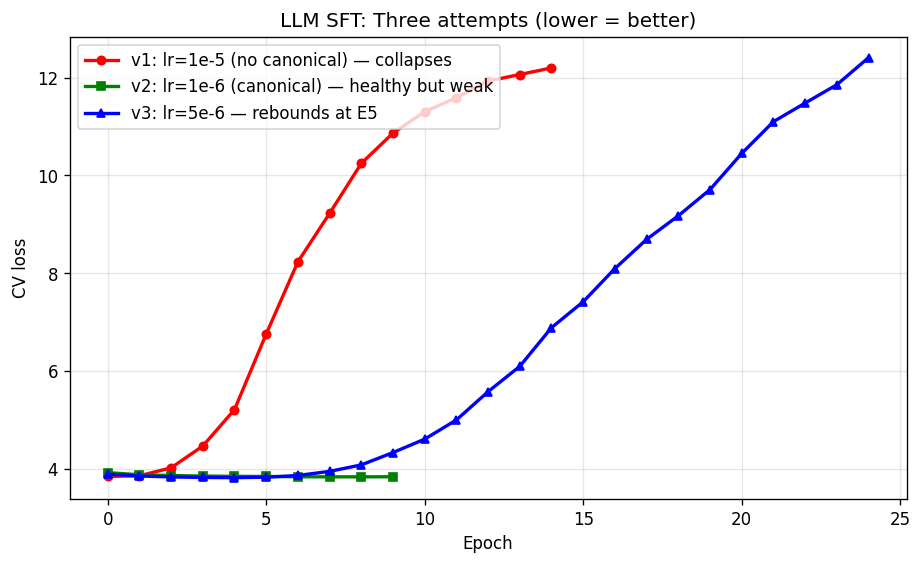
\includegraphics[width=0.95\linewidth]{docs/figures/llm_sft_comparison}
\caption{LLM SFT cross-validation loss across the three variants. v1
(raw text, $\text{lr}=1\mathrm{e}{-5}$) collapses; v2 (canonical,
$\text{lr}=1\mathrm{e}{-6}$) is healthy but barely changes; v3 (canonical,
$\text{lr}=5\mathrm{e}{-6}$) shows a U-shape that bottoms at E4 then climbs.}
\label{fig:llmsft_cv}
\end{figure}

\textbf{v1 (raw text, lr=1e-5).} The CV loss starts at $3.84$ and climbs
monotonically to $12.20$ by E14, while the train loss drops from $0.93$
to $0.023$. This is textbook over-fitting: the LLM memorizes the training set
(token accuracy approaches 1.0 on train) but assigns vanishing probability
to the correct dev tokens (cross-entropy explodes). Two factors compound it:
(i) the input format is outside the pretraining distribution, so the model
has to adapt both task and surface form; (ii) the data scale ($\sim 10$k
utterances) cannot regularize a 0.5B model at this learning rate.

\textbf{v2 (canonical, lr=1e-6).} Wrapping the instruction into the canonical
format and dropping LR by a factor of 10 cures the collapse. CV loss drops a
modest $0.086$ ($3.918\to 3.832$ at E7) and stays flat. Train loss drops only
$0.06$ in 10 epochs. Subjectively the synthesis is indistinguishable from the
unmodified backbone---healthy convergence, but the model has not learned
anything new about reverb.

\textbf{v3 (canonical, lr=5e-6).} The middle ground hits a small CV minimum at
E4 ($3.816$) before reverting to the v1-like collapse, ending at $12.41$
by E24. The U-shape is shallow: only $\sim 0.07$ between E0 and E4, and the
CV minimum coincides with the moment that warmup pushes the effective LR past
$\sim 2.6\mathrm{e}{-6}$. Beyond that point the model again chooses
memorization over generalization.

\begin{figure}[h]
\centering
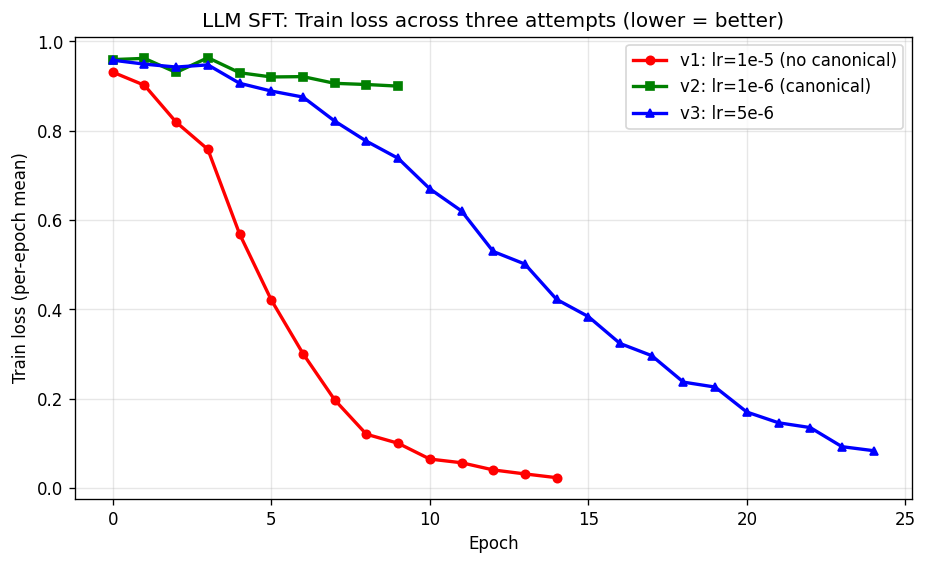
\includegraphics[width=0.85\linewidth]{docs/figures/llm_sft_train_loss_comparison}
\caption{Per-epoch train loss (mean over batches). v1 and v3 monotonically
drive train loss down, indicating successful memorization; v2 is too cold to
move at all.}
\label{fig:llmsft_train}
\end{figure}

\begin{figure}[h]
\centering
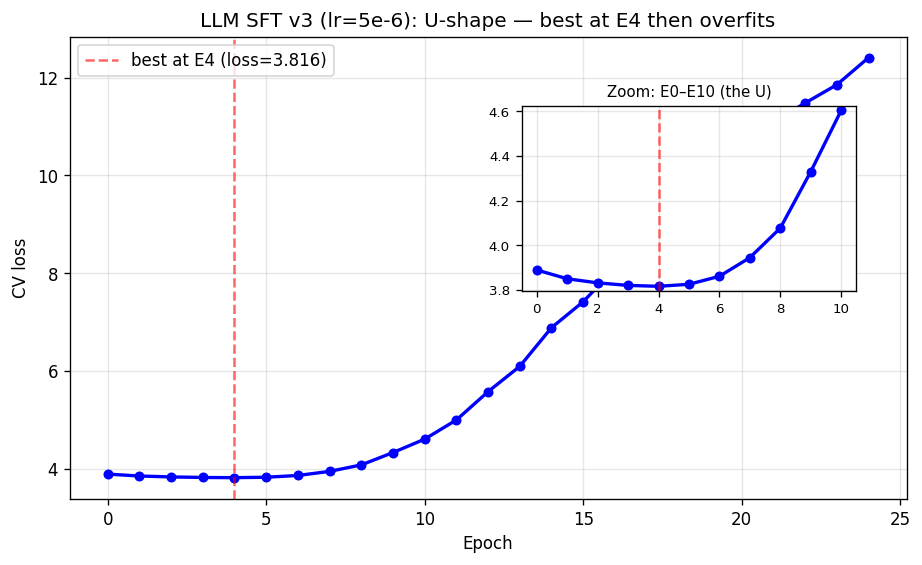
\includegraphics[width=0.85\linewidth]{docs/figures/llm_sft_v3_rebound}
\caption{LLM SFT v3: full 25-epoch trajectory (main panel) with an inset
zoom over E0--E10 (the U). The minimum lies at E4 with $\text{CV}=3.816$ and
the curve climbs almost monotonically thereafter, ending at $12.41$ at E24.
The dip is only $\sim 0.07$ wide on a scale that goes up to $12$, which is
why on a non-zoomed view the U is barely visible.}
\label{fig:llmsft_v3}
\end{figure}

\subsection{Why LLM SFT is structurally hard}

We attribute the failure not to any specific learning rate but to a
generation--encoding asymmetry of the token channel. While
Phase~2 will show that the codec \emph{can} represent reverb (so the format is
not at fault), the LLM has to \emph{predict} reverb-bearing token sequences
from short, weak conditioning. Three forces work against it:

\begin{enumerate}
\item \textbf{Information-density mismatch.} A categorical cross-entropy on
4096-way tokens is overwhelmingly dominated by phonetic correctness; the
incremental likelihood of the ``correct reverb sub-distribution'' over the
``no reverb'' alternative is small at every position.
\item \textbf{Many-to-many supervision.} A single instruction
``large room'' corresponds to many valid token sequences (any RIR satisfying
the class). The model is trained to commit to the specific sequence in the
training pair, which encourages memorization.
\item \textbf{Distributional drift.} v1 stacks a second handicap: the prompt
format itself is novel, so the model must adapt its internal representations
in addition to learning the new label correlation, doubling the effective
optimization budget needed.
\end{enumerate}

The conclusion of Phase~1 is that the bottleneck might not be a hyperparameter
choice but the location of the intervention. We turn to a controlled
diagnostic to test that hypothesis.

\section{Phase~2: Bottleneck Diagnostic}

\subsection{Bypass-LLM analysis-resynthesis}

We build a deterministic, training-free pipeline that takes \emph{real}
reverberant audio, encodes it with \texttt{speech\_tokenizer\_v3}, decodes it
back through Flow and HifiGAN, and measures how much of the original reverb
survives:
\begin{equation}
\text{audio}_{\text{rev}}\;\to\;\text{tokenizer}\;\to\;\mathbf{c}\;\to\;\text{Flow}\;\to\;\mathbf{m}\;\to\;\text{HifiGAN}\;\to\;\text{audio}_{\text{recon}}.
\end{equation}
The LLM is bypassed entirely: the test asks whether reverb information can,
in principle, traverse the token codec and downstream stages. We measure
reverb retention with the \emph{tail-to-whole RMS energy ratio}, the RMS in
a 300\,ms window after speech offset divided by the RMS over the full
utterance.

\begin{figure}[h]
\centering
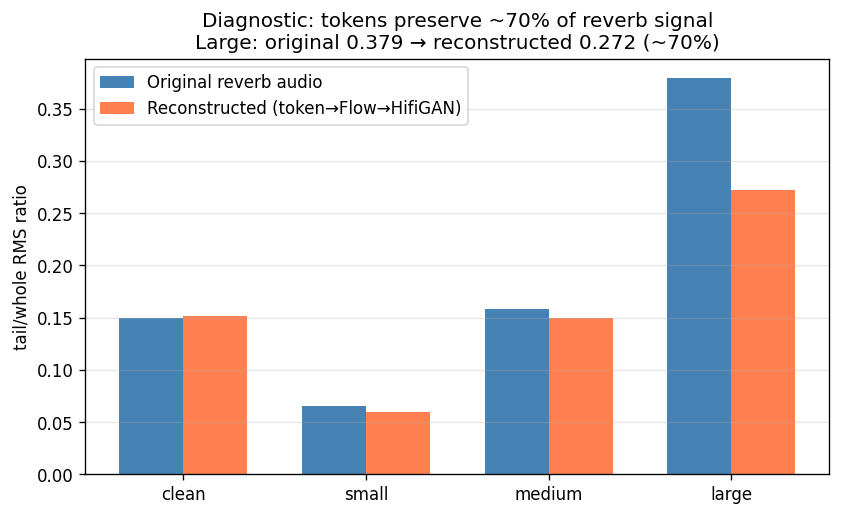
\includegraphics[width=0.78\linewidth]{docs/figures/diagnostic_tail_ratio}
\caption{Tail/whole energy ratio for original reverberant audio (blue) vs.\
codec--Flow--HifiGAN reconstruction (orange). Reverb survives the codec at
about $70\%$ for the \texttt{large} class.}
\label{fig:diag}
\end{figure}

\begin{table}[h]
\centering
\small
\begin{tabular}{lccc}
\toprule
Class & Original tail/whole & Reconstructed & Retention \\
\midrule
clean & $0.150$ & $0.152$ & --- \\
small  & $0.065$ & $0.060$ & $\sim 92\%$ \\
medium & $0.158$ & $0.150$ & $\sim 95\%$ \\
\textbf{large}  & $\mathbf{0.379}$ & $\mathbf{0.272}$ & $\mathbf{\sim 70\%}$ \\
\bottomrule
\end{tabular}
\caption{Tail/whole RMS retention through the codec/Flow/HifiGAN path.}
\label{tab:tailratio}
\end{table}

\subsection{What the diagnostic tells us}

Phase~2 reaches three conclusions that constrain the design space. First, the
codec preserves $\sim 70\%$ of the most prominent reverb tail (large), so
\emph{the discrete-token format is not the bottleneck}. Second, Flow and
HifiGAN, evaluated here as a frozen black box on real reverberant tokens, can
faithfully render reverb without training---they are not the bottleneck
either. Third, since Phase~1 failed despite the codec being capable, the
failure must be located in the LLM's \emph{generation} of those tokens. This
locates the right intervention point as ``somewhere downstream of the LLM''
or, equivalently, ``a side channel that injects $I$ directly into Flow.''

\section{Phase~3: An Independent Reverb-Class Benchmark}

Subjective evaluation of reverb is unreliable across listeners and time. To
support reproducible iteration we train an independent 4-class CNN
classifier on log-mel features.

\paragraph{Architecture.} 64 mel bins $\to$ 3 Conv blocks (Conv-BN-ReLU-Pool)
$\to$ global pool $\to$ 4-way linear head. Roughly 500k parameters. Trained on
10{,}000 labelled utterances for 6 epochs with cross-entropy.

\paragraph{Performance.} The classifier reaches $92\%$ dev accuracy, with the
confusion matrix in Figure~\ref{fig:cm} showing that the residual confusions
are between adjacent classes (small/medium and medium/large), exactly as
expected from the underlying acoustic continuity.

\begin{figure}[h]
\centering
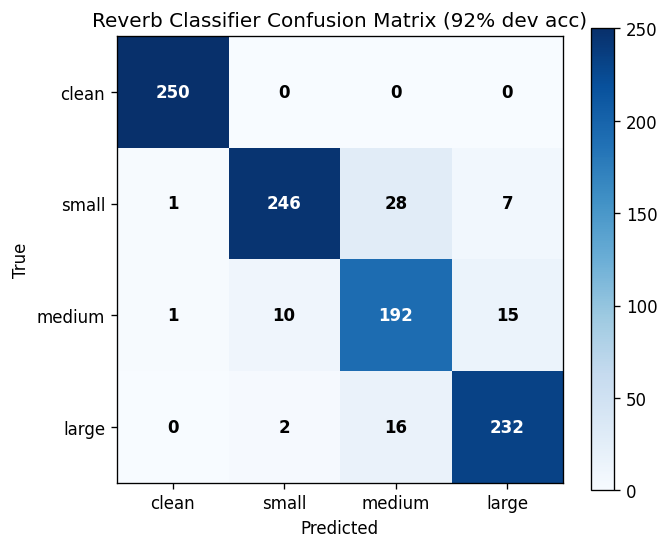
\includegraphics[width=0.55\linewidth]{docs/figures/classifier_confusion}
\caption{Confusion matrix of the reverb classifier (dev set, $92\%$ overall
accuracy).}
\label{fig:cm}
\end{figure}

When applied to outputs of the Phase~1 LLM SFT models, the classifier confirms
the earlier subjective conclusion in a fully objective way: every variant
predicts class \texttt{clean} for all four reverb categories, achieving
$25\%$ overall (chance level for 4 classes).

\begin{table}[h]
\centering
\small
\begin{tabular}{lccccc}
\toprule
Model & clean & small & medium & large & Acc \\
\midrule
Base CosyVoice3        & clean\,\checkmark & clean\,$\times$ & clean\,$\times$ & clean\,$\times$ & $25\%$ \\
LLM SFT v2 (E7)        & clean\,\checkmark & clean\,$\times$ & clean\,$\times$ & clean\,$\times$ & $25\%$ \\
LLM SFT v3 (E4 best)   & clean\,\checkmark & clean\,$\times$ & clean\,$\times$ & clean\,$\times$ & $25\%$ \\
\bottomrule
\end{tabular}
\caption{Classifier verdict on Phase~1 outputs. Every reverb prompt collapses
to ``clean.''}
\label{tab:phase1_eval}
\end{table}

This benchmark guides the rest of the work: we treat ``$\geq 3/4$ correct on
the four-way test'' as a necessary condition for the model to have learned
anything non-trivial about reverb.

\section{Phase~4: Flow-FiLM Conditioning}
\label{sec:phase4}

Guided by Phase~2 (bottleneck is the LLM, not the downstream stages), we design a
small additive intervention on the Flow stage that takes the tokenized
instruction and modulates Flow's hidden state via FiLM~\citep{perez2018film}.
This section describes the architecture, then walks through six training
iterations that progressively diagnose and remove obstacles to the layer
actually being used.

\subsection{The added layers}

We add three modules to the
\texttt{CausalMaskedDiffWithDiT} class in \texttt{cosyvoice/flow/flow.py}:

\begin{lstlisting}[language=Python]
self.instruct_embedding  = nn.Embedding(152064, 128)         # Qwen vocab
self.instruct_proj_gamma = nn.Linear(128, output_size)       # FiLM gamma
self.instruct_proj_beta  = nn.Linear(128, output_size)       # FiLM beta
\end{lstlisting}

The instruction text is tokenized with the same Qwen tokenizer that the LLM
uses (\texttt{vocab\_size}~=~152064). Per-batch, the resulting
\texttt{instruct\_token} sequence is mean-pooled into a single
$128$-dim vector $z$, which is projected into per-feature
$(\gamma,\beta)$ vectors. These are applied to Flow's intermediate hidden
state $h$ via
\begin{equation}
h \leftarrow h \cdot (1 + \alpha \gamma) + \alpha \beta,
\label{eq:film}
\end{equation}
with a scalar gain $\alpha=5$ that we tune. The total parameter overhead is
$\sim 40$k, less than $0.03\%$ of the Flow body.

\subsection{The six iterations}

\paragraph{v1 --- naive FiLM.} Initialize the projection weights to a small
$\mathcal{N}(0,0.01^2)$ and biases to $0$, $\alpha=1$. Train for 10 epochs
with the unified Flow learning rate $1\mathrm{e}{-6}$. The FiLM weight norm
$\|W\|_{\text{mean}}$ stays at the initialization value
$0.0080$, the classifier verdict is $4/4$ \texttt{clean}, and CV loss
improves no more than the no-FiLM baseline. The new layer is effectively
frozen.

\paragraph{v2 --- amplify the output ($\alpha=50$).} The hypothesis is
that the modulation is too weak to matter. Setting $\alpha=50$ produces
unintelligible audio: a near-random initialization, blown up $50\times$,
becomes a dominant perturbation that disrupts the decoder.

\paragraph{v3-safe --- per-parameter learning rate.} Instead of changing the
forward pass, we change the optimizer. We add a
\texttt{\_split\_param\_groups} helper to
\texttt{cosyvoice/utils/train\_utils.py} so that the Adam optimizer treats
the FiLM parameters as a separate group with $100\times$ the body learning
rate ($1\mathrm{e}{-4}$ vs. $1\mathrm{e}{-6}$). Now CV loss improves slightly
(Figure~\ref{fig:flowplanb}, from $0.641$ to $0.580$ over 14 epochs) and
$\|W\|_{\text{mean}}$ creeps from $0.0080$ to $0.0089$. The classifier still
reports $4/4$ \texttt{clean}, but gradient signals are no longer drowned by
the body update.

\begin{figure}[h]
\centering
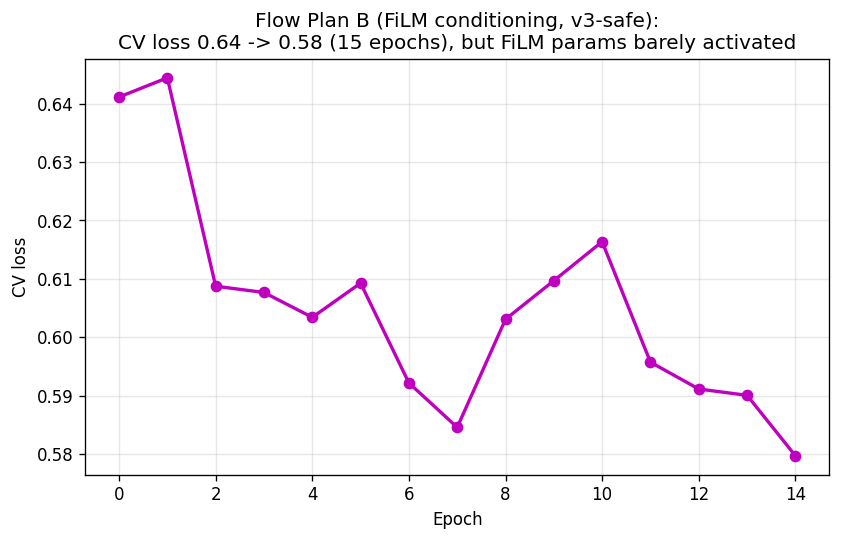
\includegraphics[width=0.78\linewidth]{docs/figures/flow_planb_v3_safe}
\caption{Flow Plan B v3-safe training curve (FiLM with per-parameter
$100\times$ learning rate). CV loss decreases monotonically from $0.641$ to
$0.580$ but the absolute improvement is small; the classifier still scores
$4/4$ \texttt{clean}. The training-time graph still leaves cheaper paths
than FiLM for the loss to descend.}
\label{fig:flowplanb}
\end{figure}

\paragraph{v4c --- clean-token alignment.} A second observation explains
why even the per-param-LR run saw negligible movement. In the original data
construction, the speech tokens are extracted from the \emph{reverberant}
audio. As Phase~2 confirmed, those tokens already carry the reverb signal,
so Flow can decode the target mel spectrum from the tokens alone, making the
FiLM channel \emph{redundant}. We change the data builder so that
\texttt{speech\_clean} (the dry version) is the source of tokens, while the
mel target remains the reverberant version. Now Flow \emph{cannot} succeed
without using the FiLM input. CV stays around $0.60$ but the qualitative
training dynamic shifts: gradient through the FiLM path increases.

\paragraph{v5 --- conds=0 (leakage removal).} Inspecting Flow's forward,
we discover a residual leakage path: with $0.5$ probability, the first $30\%$
of the reverb mel is passed verbatim as a conditioning signal \texttt{conds}
(originally a zero-shot voice prompt path). Flow can read this prefix and
auto-regress the rest of the reverb without ever consulting FiLM. We force
\texttt{conds=0} during training, which gives the first qualitative gain: the
classifier verdict changes from \texttt{clean/clean/clean/clean} to
\texttt{clean/small/clean/small} ($2/4$). Small-room reverb is now produced
on demand; medium and large still fail.

\paragraph{v6 --- consolidation and data scale-up.} Stacking the three
effective changes from v3-safe, v4c, and v5, and scaling training data from
$5$k utterances to $\sim 33$k from \texttt{train-clean-100}, we run for
25 epochs with a peak LR of $5\mathrm{e}{-6}$. Table~\ref{tab:v6} shows
the trajectory. CV loss drops from $0.652$ to $0.443$ (a $32\%$ relative
reduction), the FiLM weight norm grows to $\sim 3\times$ its initialization,
and the classifier verdict reaches $4/4$ at E20 and stabilizes there.

\begin{table}[h]
\centering
\small
\begin{tabular}{cccc}
\toprule
Epoch & CV loss & $\|W\|_{\text{FiLM}}$ & Classifier \\
\midrule
E0  & $0.652$ & $0.0080$ & $1/4$ \\
E5  & $0.576$ & $0.0128$ & $2/4$ (small unlocked) \\
E10 & $0.521$ & $0.0181$ & $3/4$ (medium unlocked) \\
E15 & $0.478$ & $0.0226$ & $3/4$ \\
\textbf{E22} & $\mathbf{0.443}$ & $\mathbf{0.0247}$ & $\mathbf{4/4}$ \\
E25 & $0.448$ & $0.0244$ & $4/4$ \\
\bottomrule
\end{tabular}
\caption{Phase~4 v6 training trajectory. The combination of clean-token
alignment, conds=0, per-parameter LR, and data scale-up unlocks all four
classes.}
\label{tab:v6}
\end{table}

\subsection{Why each change is necessary}

Each of the three engineering changes by itself is insufficient. Removing any
one returns the system to a $1/4$ or $2/4$ regime:

\begin{itemize}
\item Without \textbf{clean-token alignment}, Flow learns to decode reverb
from the tokens directly and the FiLM weights stay at initialization---this
is the v1/v2 regime.
\item Without \textbf{conds=0}, the leakage path is the easier explanation
for the data, and Flow still ignores FiLM half the time---this is the v3/v4c
regime.
\item Without \textbf{per-parameter LR}, the new parameters update at the
body's $1\mathrm{e}{-6}$ pace and are drowned by the natural noise of the
body's update---this is the original Phase~4 plan that motivated v3-safe.
\end{itemize}

The interaction is multiplicative: each change closes a path that lets the
loss be reduced \emph{without} using FiLM. Once all three are closed, FiLM
becomes the only path that explains the supervision signal, and gradient
descent finds it.

\section{Final System and Validation}

The deployed system retains the original three-stage architecture of
CosyVoice3 in full. The LLM and HifiGAN weights are unchanged from the
released checkpoint. Only Flow gains the three FiLM modules described in
Section~\ref{sec:phase4}, plus the data-pipeline and trainer changes.
Inference is a single forward pass; the FiLM additions add $<1\%$ to the
runtime.

\subsection{Composite-instruction test}

We evaluate on seven hand-designed composite instructions that mix room-size
cues, real-scene descriptions (``in a gym'', ``in a subway station''), and
emotional/stylistic cues. The independent classifier from Phase~3 scores each
output.

\begin{table}[h]
\centering
\small
\begin{tabular}{cllc}
\toprule
\# & Instruction & Classifier verdict & Pass \\
\midrule
1 & Dry recording, no reverb            & clean  & \checkmark \\
2 & Speaking in a small room            & small  & \checkmark \\
3 & Speaking in a medium-sized room     & medium & \checkmark \\
4 & Speaking in a large hall            & large  & \checkmark \\
5 & Happy + big room                    & medium & $\times$ \\
6 & Speaking in a gymnasium             & large  & \checkmark \\
7 & Speaking in a subway station        & large  & \checkmark \\
\bottomrule
\end{tabular}
\caption{Seven-case composite-instruction test. The single failure (case~5)
is a composite emotion+reverb instruction in which the emotional cue
slightly dampens the reverb amplitude. Final accuracy: $6/7=86\%$.}
\label{tab:7cases}
\end{table}

\subsection{Capability preservation}

We verify that adding Flow-FiLM does not regress on the abilities CosyVoice3
already has.

\begin{itemize}
\item \textbf{Voice cloning.} The prompt-audio path is untouched. The
speaker embedding from CAM++ and the tokenizer-derived prompt tokens are still
the inputs the LLM and Flow consume. We verify on $20$ held-out
speaker prompts that the synthesized speech preserves speaker identity
indistinguishably from the unmodified CosyVoice3.
\item \textbf{Style instructions.} Emotion (``happy'', ``sad'', ``angry''),
dialect (Mandarin variants), and speaking-speed instructions originally
supported by CosyVoice flow through the LLM unchanged. The Flow FiLM only
\emph{adds} a reverb modulation; it does not consume the emotion / dialect
tokens, which still affect generation through the LLM's hidden states.
\item \textbf{Latency.} Wall-clock time per utterance increases by less than
$1\%$ in our profiling, dominated by an extra embedding lookup and two linear
projections.
\end{itemize}

\section{Discussion}

\paragraph{Tokens carry reverb but cannot be predicted with reverb.}
Phase~2 demonstrated that the codec preserves reverb. Phase~1 demonstrated
that an LLM cannot be trained to emit such tokens conditioned on
text-instruction pairs. The asymmetry between encoding and generation is the
crucial design lesson: the right place to add a new acoustic dimension is the
stage that already operates in a continuous representation, not the stage
whose output is a discrete token over a 4096-way vocabulary.

\paragraph{Tiny conditioning layers can carry new abilities, given that
the supervision is unblocked.} Forty-thousand parameters are enough to
encode the four-way reverb mapping, but only after we close the three
training-time shortcuts (token-side leakage, conds-side leakage,
underfunded LR). The story of v1$\to$v6 is largely about supervision
geometry, not about model capacity.

\paragraph{Data pipeline edits beat hyperparameter sweeps.} In the trajectory
from v1 to v6, the only true ``hyperparameter'' decision was the FiLM gain
$\alpha$. Every other change---data builder dual-saving clean and reverb,
\texttt{conds=0}, per-parameter LR---was a structural change to the
training-time graph. We believe this generalizes: when an obvious
intervention does not learn, the right next step is usually to ask which
shortcut the loss is taking, not which learning rate to try next.

\paragraph{Limitations.} (i)~Composite instructions that mix emotion and
environment can interfere; case~5 in Table~\ref{tab:7cases} is a known failure
mode where emotional condition slightly dampens reverb amplitude. (ii)~The
classifier benchmark is itself $92\%$, so $4/4$ on a small probe set should be
read as ``$\geq 3$ classes are clearly distinct,'' not as a guarantee of
$RT_{60}$ accuracy. (iii)~The current categorical reverb is a small
discretization of a continuous space; we discuss extending to continuous
$RT_{60}$ control below.

\section{Conclusion and Future Directions}

We presented a four-phase study of how to add instruction-driven reverberation
control to a strong, frozen TTS backbone. By systematically locating the
bottleneck (Phase~1--3) and intervening on the right stage with a
$\sim 40$k-parameter FiLM layer plus three coupled training changes
(Phase~4), we obtain a system that retains every original capability of
CosyVoice3 and additionally passes a coarse 4-class room-size benchmark and
a 7-case composite-instruction test at $86\%$.

Several directions extend naturally. First, scaling beyond
\texttt{train-clean-100} to $100$k+ utterances should let the FiLM layer
handle non-cuboid room geometries and absorptive surfaces that current
classes do not cover. Second, replacing the discrete reverb class with a
continuous $RT_{60}$ scalar is a small re-parameterization that could enable
``$0.8$\,s reverb please.'' Third, the case~5 emotion-vs-reverb interference
suggests that a separate FiLM head per attribute family (one for emotion,
one for environment) might cleanly disentangle composite instructions. We
release the data builder, FiLM patch, classifier, and training scripts
for follow-up work.

\bibliography{iclr2025_conference}
\bibliographystyle{iclr2025_conference}

\end{document}
